\documentclass[11pt,a4paper]{article}
\usepackage[margin=23mm]{geometry}
\usepackage[T1]{fontenc}
\usepackage{lmodern,microtype}
\usepackage{amsmath,booktabs,graphicx}
\usepackage{caption}
\usepackage[hidelinks]{hyperref}
\setlength{\parindent}{0pt}
\setlength{\parskip}{5pt}
\clubpenalty=10000
\widowpenalty=10000
\captionsetup{font=small,labelfont=bf}
\graphicspath{{figures/}}
\title{ID2223 Lab 1: Convolutional Neural Networks\\[0.5em]\large Group name: THE MEGA BEST GROUP}
\author{Riccardo Fragale, Lorenzo Deflorian, Siyue Zhang}
\date{23 November 2026}
\begin{document}
\maketitle

In this task we trained AlexNet and ResNet-18 on CIFAR-10 and compared their accuracy, robustness and cost. We didn't attempt the optional challenges.

\section{Task 1: Data preparation}
Each image in the dataset is a $32\times32$ RGB photo with one label from ten classes, such as airplane, cat, truck or others. The training set has 50,000 images, 5,000 per class. 
We use a stratified split with seed 2223: 45,000 training and 5,000 validation images, so each class has 500 validation images. CIFAR-10 is balanced, so no class reweighting is needed. Stratification preserves this balance in training and validation.
The fixed seed has been used to ensure reproducibility.
The official 10,000 test images are kept for final evaluation(test).

Both models use the same preprocessing. Pixels are scaled to $[0,1]$ and normalized with the training split's channel means and standard deviations. Computing normalization statistics only from the training partition avoids data leakage.
We keep the $32\times32$ size because both architectures are adapted to small images. We seed Python, NumPy, PyTorch and the training DataLoader, and use deterministic cuDNN settings on CUDA.

\section{Task 2: Models and training}
We build both models from PyTorch layers without pretrained weights. 
The original AlexNet was built for about $224\times224$ images and starts with an $11\times11$, stride-4 convolution.
On $32\times32$ images this would shrink the feature maps too quickly, so we follow the Part A9 adaptation. 
Our AlexNet has five $3\times3$ convolutions with 64, 192, 384, 256 and 256 channels. Each uses stride 1, padding 1 and ReLU. 
Three max-pooling layers reduce the image size from 32 to 16, 8 and 4, so the last feature map is $256\times4\times4$. 
The classifier has sizes $4096\rightarrow1024\rightarrow512\rightarrow10$, with dropout 0.5 in its two hidden layers.
It is smaller than the original classifier, and we leave out local response normalization.

For the same reason, ResNet-18 starts with a $3\times3$ stride-1 convolution instead of the original $7\times7$ stride-2 convolution and max-pool. It has four stages of two residual blocks, with widths 64, 128, 256 and 512. The last three stages halve the spatial size, ending at $512\times4\times4$. Global average pooling and a linear layer give ten logits. Each block adds its input back through a shortcut, using a $1\times1$ convolution when the shapes differ. The shortcut gives gradients a direct path to earlier layers, which makes a deeper network easier to train. ResNet also differs from our AlexNet in width and batch normalization, so this comparison does not isolate the effect of the shortcuts.

Both networks at training time use cross-entropy and SGD with learning rate 0.01, momentum 0.9, cosine decay and batch size 64. 
The baselines have no augmentation or weight decay.
We saved the checkpoint with the highest validation accuracy and break ties with lower loss. 
We decided a compute budget of 20 epochs, or 900,000 training examples ($45{,}000\times20$), for every run.

\begin{table}[htbp]
\centering
\caption{Task 2 results from the November 18 Mac MPS run, at the selected epoch. Time covers all 20 epochs.}
\label{tab:baseline}
\begin{tabular}{lrr}
\toprule
 & AlexNet & ResNet-18\\
\midrule
Parameters & 6,976,842 & 11,173,962\\
Selected epoch & 17 & 18\\
Validation accuracy (\%) & 83.84 & 85.74\\
Validation loss & 0.880 & 0.677\\
Training accuracy (\%) & 99.78 & 100.00\\
Training time (min) & 4.95 & 12.94\\
\bottomrule
\end{tabular}
\end{table}

In Table~\ref{tab:baseline}, ResNet gains 1.90 points in validation accuracy but takes about 2.6 times as long to train. Both models almost perfectly fit the training data, while their validation accuracy is 14 to 16 points lower. This gap shows overfitting.

\section{Task 3: Capacity and regularization}
We change one AlexNet setting at a time. The baseline uses width 1.0, dropout 0.5 and no weight decay. All runs keep the same split, seed, optimizer, batch size and 20-epoch budget, with no augmentation. The same baseline run is used in the width, L2 and dropout comparisons.

These comparisons investigate whether changing capacity or regularization improves generalization within our training budget. Varying width measures the accuracy gained for extra parameters and training time, while L2 and dropout test whether we can reduce overfitting without enlarging the model. Changing one factor at a time helps attribute differences to that setting.

\begin{table}[htbp]
\centering\small
\caption{Task 3 results reported in the notebook for the November 19 Mac MPS run. Metrics are at the selected checkpoint. Time covers all 20 epochs.}
\label{tab:sweep}
\begin{tabular}{lrrrrr}
\toprule
Setting & Params (M) & Val. (\%) & Val. loss & Train (\%) & Time (min)\\
\midrule
Baseline & 6.98 & 83.84 & 0.880 & 99.78 & 4.31\\
Width 0.5 & 1.75 & 82.00 & 0.804 & 98.04 & 2.08\\
Width 1.5 & 15.69 & 84.54 & 0.883 & 99.97 & 7.94\\
L2 $10^{-4}$ & 6.98 & 84.12 & 0.785 & 99.47 & 4.40\\
L2 $10^{-3}$ & 6.98 & 84.24 & 0.580 & 98.16 & 4.19\\
Dropout 0 & 6.98 & 82.78 & 1.209 & 100.00 & 4.08\\
Dropout 0.25 & 6.98 & 83.36 & 0.992 & 99.92 & 4.09\\
\bottomrule
\end{tabular}
\end{table}

In Table~\ref{tab:sweep}, the smaller model roughly halves training time but loses 1.84 accuracy points. The wider model gains only 0.70 points and takes 7.94 minutes, using about 2.25 times as many parameters as the baseline. Even width 0.5 reaches 98\% training accuracy, so none of the settings clearly underfits. The notebook's learning curves show signs of overfitting for all three widths after roughly epoch 10: training loss approaches zero while validation loss rises. More capacity therefore provides a modest accuracy gain at a substantial cost without resolving overfitting.

L2 at $10^{-3}$ lowers validation loss from 0.880 to 0.580 at about the same cost and keeps validation loss flatter late in training. Its slightly lower training accuracy of 98.16\%, together with improved validation performance, is consistent with effective regularization. Removing dropout gives the highest validation loss in the dropout comparison, even though training accuracy reaches 100\%; its validation loss rises to about 1.27 by epoch 20. Dropout 0.25 falls between no dropout and 0.5, supporting the use of head dropout under this budget.

All configurations reduce training loss sharply within 20 epochs, suggesting that overfitting is a bigger problem than stalled optimization. Among the tested single-factor changes, L2 at $10^{-3}$ offers the strongest validation-loss improvement and a modest accuracy gain at approximately the baseline's training cost. Width 1.5 gives the highest validation accuracy, but its extra cost makes regularization the more economical improvement in these runs.

\section{Task 4: Augmentation and robustness}
We decided to use AlexNet for task 4 as generally data augmentation helps when the model is overfitting data in a normal training and AlexNet seemed the one having more this issue in the previous stages of the lab.
We would like to add some ability to generalize to the model.
We will call below the baseline AlexNet as\emph{Original} and the version trained with data augmentation \emph{Augmented}. Augmented uses random crops after four pixels of reflection padding, plus horizontal flips with probability 0.5. 
These changes keep the objects still recognizable while varying their position in the grid(of 32 x 32 pixels) and left-right orientation. Validation images are not augmented.

Both models are tested on the same 5,000 validation images. 
We add Gaussian noise, rotate images or apply a $5\times5$ Gaussian blur, each at two strengths. 
Each "corruption" is applied on its own to the $[0,1]$ pixels, before normalization. 
The noise is fixed for each image, so both models see the same noisy images. Rotation uses bilinear interpolation and black fill.

\begin{table}[htbp]
\centering
\caption{Validation accuracy on the same 5,000 images, evaluated on an RTX 3050 Ti GPU. A shared run gave 56.14\% for Original at $\sigma=0.10$; the notebook traces this one-image difference to cuDNN TF32.}
\label{tab:robustness}
\begin{tabular}{lrr}
\toprule
Condition & Original (\%) & Augmented (\%)\\
\midrule
Clean & 84.30 & 87.28\\
Noise, $\sigma=0.05$ & 78.48 & 77.10\\
Noise, $\sigma=0.10$ & 56.16 & 46.44\\
Rotation, $10^\circ$ & 66.48 & 74.00\\
Rotation, $25^\circ$ & 40.14 & 50.02\\
Blur, $\sigma=0.5$ & 81.38 & 84.38\\
Blur, $\sigma=1.0$ & 53.58 & 53.24\\
\bottomrule
\end{tabular}
\end{table}

Augmentation helps on clean images, rotation and mild blur (Table~\ref{tab:robustness}). Under strong noise it loses 9.72 points. Strong blur gives similar results for both models.

Noise and blur hide fine details, and rotation cuts off the corners of the image. Under strong noise, most wrong predictions are frog: 1,886 of 2,678 errors for Augmented and 1,323 of 2,192 for Original. Augmented predicts frog much more often, which explains most of its lower noise accuracy. Under rotation and strong blur, cat is the most common wrong prediction, at 44 to 60\% of errors.

Augmented took 9.29 minutes to train and Original took 9.05 minutes. Augmentation added 14.65 seconds, about 2.7\%, for a 2.98-point gain on clean images. Given the small size of the model
and the reduced time to train it we think it's an affordable time increase.

\section{Task 5: Predictions and adversarial examples}
In this task, we investigate what the models get right and wrong, and whether small, deliberately chosen pixel changes can alter their predictions. We compare Original and Augmented using class-level results, representative predictions and training curves, then generate adversarial examples against both models. This extends Task 4's corruption tests by distinguishing sensitivity to random changes from sensitivity to perturbations optimized to increase the model's loss.

Augmented also lowers clean validation loss from 0.890 to 0.374. Cat has the lowest recall for both models. Its recall rises from 71.2\% to 73.2\%. Total cat/dog confusions fall from 116 to 109, though cat-to-dog errors increase from 59 to 66. Frog recall improves from 85.0\% to 91.0\%.

For Original's four lowest-recall classes, Figure~\ref{fig:examples} shows the first correct and the first wrong prediction. The notebook shows the same analysis for Augmented and both confusion matrices. Original labels cat image 39 as a deer with almost 100\% confidence. Confident errors like this receive a large cross-entropy penalty. This helps explain Original's high validation loss.

\begin{figure}[!htb]
\centering
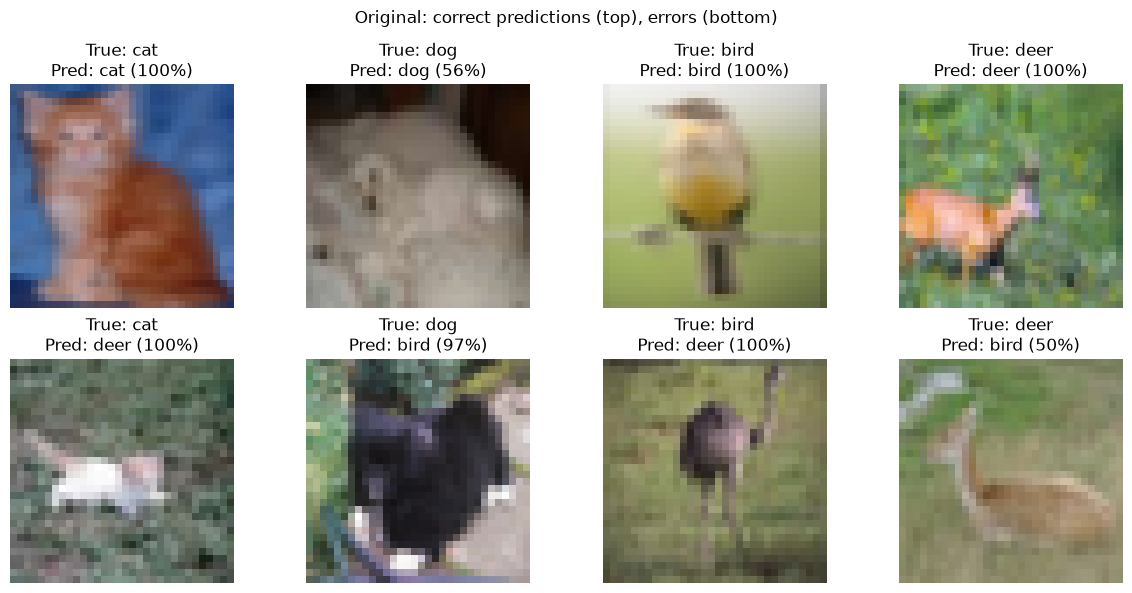
\includegraphics[width=0.78\linewidth]{prediction_examples_1.png}
\caption{Original: correct predictions in the top row and errors in the bottom row.}
\label{fig:examples}
\end{figure}

In clean evaluation mode, Original gets 99.98\% training accuracy and Augmented gets 92.67\%. Their training/validation gaps are 15.68 and 5.39 points, which supports reduced overfitting with augmentation. Augmented's training log reports 90.44\% at epoch 20. The log uses dropout, augmented images and changing weights. Its training accuracy is therefore not directly comparable to the clean evaluation.

In Figure~\ref{fig:curves}, Original's validation loss rises from 0.590 at epoch 10 to 0.890 at epoch 20, while training loss falls. Validation accuracy still improves from 81.66\% to 84.30\%, so our accuracy rule selects epoch 20. Augmented's validation loss keeps falling, from 0.420 at epoch 15 to 0.374 at epoch 20. It may benefit from more training.

\begin{figure}[!htb]
\centering
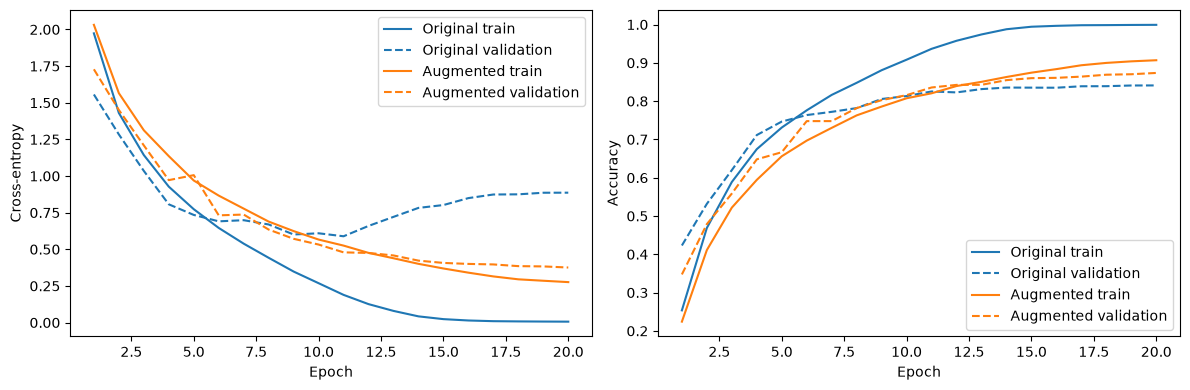
\includegraphics[width=0.95\linewidth]{learning_curves_1.png}
\caption{Training and validation curves for the November 20 AlexNet runs. Training metrics use training mode; validation uses clean images in evaluation mode.}
\label{fig:curves}
\end{figure}

We use a one-step FGSM attack with $\epsilon=4/255$. We take the sign of the loss gradient with respect to the raw pixels, add $\epsilon$ times that sign, and clip to $[0,1]$. Normalization stays inside the gradient calculation. The largest recorded pixel change is 0.0156863, which matches $4/255$ up to rounding.

We attack the first 256 validation images using each model's own gradients. As a control, both models also receive the same random signs with the same size and clipping. An attack succeeds if a correct clean prediction becomes wrong.

\begin{table}[htbp]
\centering
\caption{Results on the 256-image subset. Success rate uses only initially correct predictions.}
\label{tab:attack}
\begin{tabular}{lrrrr}
\toprule
Model & Clean (\%) & Random (\%) & FGSM (\%) & Success\\
\midrule
Original & 89.06 & 88.28 & 26.56 & 160/228 (70.18\%)\\
Augmented & 91.02 & 91.02 & 21.88 & 177/233 (75.97\%)\\
\bottomrule
\end{tabular}
\end{table}

FGSM causes many errors, while random signs have little effect (Table~\ref{tab:attack}). The control uses the same images and the same $\epsilon$, so the gap between the Random and FGSM columns shows the effect of following the gradient. Figure~\ref{fig:attack} shows Original changing its prediction from truck to automobile. The notebook also shows a truck-to-ship attack on Augmented. Crop-and-flip training did not improve resistance to FGSM in this test. The subset is small and not stratified, so these results do not measure general adversarial robustness.

\begin{figure}[!htb]
\centering
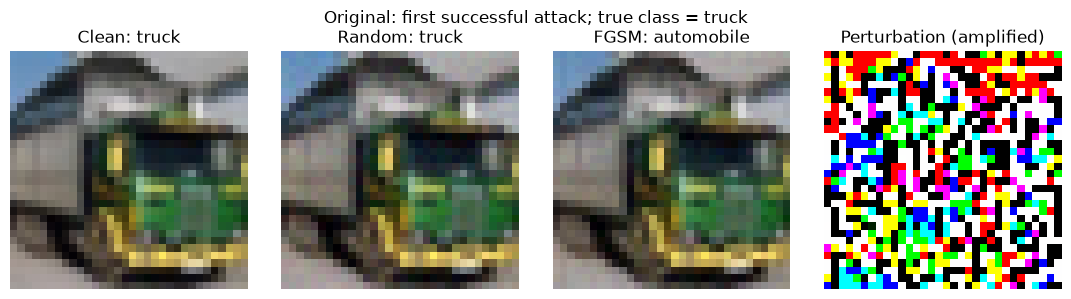
\includegraphics[width=0.8\linewidth]{fgsm_examples_1.png}
\caption{Original's first successful FGSM example. The final panel makes the small pixel changes visible by amplifying them.}
\label{fig:attack}
\end{figure}

\section{Task 6: Cost and model choice}
The final task brings together accuracy, robustness and computational cost to recommend a configuration under our 20-epoch training budget. We compare the recorded training costs and benchmark inference for the available AlexNet checkpoints at batch sizes 1 and 64. These measurements help assess both the cost of training a model and its cost during use. We also consider how training duration, randomness and hardware limit the conclusions.

We would choose Augmented for mostly clean or rotated images. It has the best validation accuracy in these runs (Table~\ref{tab:cost}) at a small extra training cost. Original is better under the tested Gaussian noise. ResNet takes about 3.7 times as long as Original for a 0.40-point gain. It had no augmentation, so its comparison with Augmented is not fully fair. In Task 3, L2 at $10^{-3}$ took about the same training time as the baseline. Width 1.5 took about 1.84 times as long for a 0.70-point gain.

\begin{table}[!htb]
\centering
\caption{November 20 runs, each trained for 20 epochs. Validation accuracy is from the best checkpoint.}
\label{tab:cost}
\begin{tabular}{lrrr}
\toprule
Model & Params (M) & Val. accuracy (\%) & Training (min)\\
\midrule
Original AlexNet & 6.98 & 84.30 & 9.05\\
Augmented AlexNet & 6.98 & 87.28 & 9.29\\
ResNet-18 & 11.17 & 84.70 & 33.52\\
\bottomrule
\end{tabular}
\end{table}

Without the November 20 ResNet weights, we only measure inference and robustness for the two AlexNet models. We time inference on an RTX 3050 Ti Laptop GPU with float32 inputs and cuDNN TF32 enabled. For each model and batch size, we run six trials and alternate the model order. Each trial has five warm-up passes and 20 timed passes. We synchronize the GPU before and after timing. Times exclude loading, preprocessing, transfers and metric calculations.

\begin{table}[htbp]
\centering
\caption{Median inference time per batch. IQR is the 25th to 75th percentile of the six trial means.}
\label{tab:timing}
\begin{tabular}{lrrr}
\toprule
Model & Batch size & Median (ms) & IQR (ms)\\
\midrule
Original & 1 & 2.60 & 2.57--2.81\\
Augmented & 1 & 2.71 & 2.45--2.91\\
Original & 64 & 4.78 & 4.77--4.96\\
Augmented & 64 & 4.84 & 4.78--4.97\\
\bottomrule
\end{tabular}
\end{table}

Both AlexNet models have the same architecture and checkpoints of about 26.62 MiB. Their measured inference times are similar (Table~\ref{tab:timing}). Batch 64 processes about 13,000 images per second, compared with fewer than 400 at batch 1.

ResNet beats AlexNet in both runs, but its gain falls from 1.90 points on November 18 to 0.40 points on November 20. AlexNet's training time rises from 4.95 to 9.05 minutes. Both runs use the same seed and split. These single-run results do not show variation across seeds.

The training budget may also change the ranking. Augmented is still improving at epoch 20. ResNet peaks at 84.70\% at epoch 15 and ends at 84.46\%. Next, we would train ResNet with the same crop-and-flip augmentation for a fairer comparison. We would also test mild noise augmentation under the same budget.

\end{document}
